\documentclass[a4paper,french,oneside,10pt]{book}
\usepackage[utf8]{inputenc}
\usepackage{lettrine}
\usepackage{float} 
\usepackage[french]{babel}
\usepackage{fancyhdr}
\usepackage{enumerate}
\usepackage{graphicx}
\usepackage{multirow}
\usepackage{listings}
\usepackage{color}
\usepackage{placeins}
\usepackage{tabularx}
\usepackage[french,ruled,vlined,linesnumbered]{algorithm2e}
\usepackage{amsmath}
\usepackage{amssymb}
\usepackage[bookmarks=true]{hyperref}
\hypersetup{pdfborder={0 0 0}}
\pagestyle{fancy}
\setlength{\parskip}{1.5ex plus .4ex minus .4ex}
\renewcommand{\labelitemi}{\textbullet}
\renewcommand{\chaptermark}[1]{\markboth{#1}{}}



\pagestyle{fancy}

\renewcommand{\chaptermark}[1]{\markboth{#1}{}}
\renewcommand{\sectionmark}[1]{\markright{\thesection\ #1}}

\fancyhf{}

\fancyhead[RO,LE]{\thepage}
\fancyhead[LO]{\leftmark}
\fancyhead[RE]{Projet GMIN103 Base de données avancée}

\fancypagestyle{corps}{ 
\fancyhead[RO,LE]{\thepage}
\fancyhead[LO]{\rightmark}
\fancyhead[RE]{\leftmark}
}

\renewcommand{\footrulewidth}{0pt} % pas de filet en bas
\fancypagestyle{plain}{ % pages de tetes de chapitre
\fancyhead{}
% supprime l’entete
\renewcommand{\headrulewidth}{0pt} % et le filet
}
\newcommand{\clearemptydoublepage}{%
	\newpage{\pagestyle{empty}\cleardoublepage}}


%Modification des marges
%\\oddsidemargin}{-2,5cm}
%\addtolength{\textwidth}{5cm}
%\addtolength{\topmargin}{-2,5cm}
%\addtolength{\textheight}{4cm}

%definition des fonctions de la page de garde
\def\blurb{%
  \begin{tabular}{l p{0.6cm} c p{0.8cm} r}
   \multirow{3}{*}{\vspace{-1.5cm}\hspace{-1cm}
\includegraphics[width=3cm]{./files/um2}} & & & &  \multirow{3}{*}{\vspace{-1.5cm}
\includegraphics[width=2cm]{./files/ufr}} \\
    & & Ministère de l'Éducation Nationale & & \\
    & & Université de Montpellier II & & \\ 
    & & Place Eugène Bataillon & & \\ 
    & & 34095 Montpellier Cedex 5 & & \\ 
    \vspace{0.5cm}
   \end{tabular}
  }
\def\clap#1{\hbox to 0pt{\hss #1\hss}}%
\def\ligne#1{%
  \hbox to \hsize{%
    \vbox{\centering #1}}}%
\def\haut#1#2#3{%
  \hbox to \hsize{%
    \rlap{\vtop{\raggedright #1}}%
    \hss
    \clap{\vtop{\centering #2}}%
    \hss
    \llap{\vtop{\raggedleft #3}}}}%
\def\bas#1#2#3{%
  \hbox to \hsize{%
    \rlap{\vbox{\raggedright #1}}%
    \hss
    \clap{\vbox{\centering #2}}%
    \hss
    \llap{\vbox{\raggedleft #3}}}}%

%definition du titre et autres param
\def\titre{\LARGE Projet GMIN103 Base de données avancée \\ Thésaurus Rex}
\def\sstitre{Rapport (Décembre 2011)}
\def\auteurs{
	  Baptiste \textsc{Le Bail} \\
      Thibaut \textsc{Marmin} \\
      Namrata \textsc{Patel} \\
      Clément \textsc{Sipieter} \\
      Steeve \textsc{Tuvée}}


\begin{document}

% Def variable coloration code source
\definecolor{keyword}{rgb}{0.55,0,0} 
\definecolor{type}{rgb}{0,0.55,0} 
\definecolor{comment}{rgb}{0.7,0.7,0.7} 

\lstset{
basicstyle=\scriptsize\sffamily,
numbers=left,
numberstyle=\scriptsize\color{comment},
keywordstyle=\color{keyword}\bfseries,
commentstyle=\color{comment},
breaklines=true,
fontadjust=true,
columns=fullflexible,
morekeywords=true
}

\lstset{emph={ varchar , integer , bigint , date , smallint , real , OLD , NEW , plpgsql , ROWTYPE, int},
emphstyle=\color{type}}



\frontmatter
\renewcommand{\labelitemii}{\textasteriskcentered}
\thispagestyle{empty}
  \vbox to .9\vsize{%
  \vss
  \vbox to 1\vsize{%
    \haut{}{\blurb}{}
    \vfill
    
    \noindent\rule{\linewidth}{.5pt}
    \ligne{\vspace{1.5mm}\titre}
    \noindent\rule{\linewidth}{.5pt}
    \ligne{\normalsize{\textsc{\sstitre}}}
    \vfill
    \ligne{%
      \begin{tabular}{l}
	\vspace{5mm}
      \end{tabular}
      \begin{tabular}{c}
      Travail réalisé par : \\\\
       \auteurs
      \end{tabular}
    }
        \ligne{%
      \begin{tabular}{l}
	\vspace{15mm}
      \end{tabular}
      \begin{tabular}{c}
      \texttt{https://github.com/marminthibaut/bdd\_projet/}
      \end{tabular}
    }
  \vss
  }
}
\clearemptydoublepage
\chapter*{Introduction}
Un thésaurus est un type de langage documentaire qui constitue un vocabulaire normalisé. Il regroupe de manière organisée les termes d'un même domaine de connaissance. Cet outil linguistique permet de décrire des concepts et de lever les ambiguïtés induites par les relations de synonymie, d'homonymie et de polysémie présentes dans le langage naturel.

L'outil développé lors de ce projet sera composé de termes décrivant des concepts, reliés entre eux par des relations hiérarchiques, synonymiques et associatives. L'utilisateur aura la possibilité d'explorer la hiérarchie et de gérer (ajouter / modifier / supprimer) les termes et les concepts.

Ce travail, réalisé par une équipe de cinq étudiants\footnote{Baptiste Le Bail, Thibaut Marmin, Namrata Patel, Clément Sipieter, Steeve Tuvée}, est présenté dans ce rapport selon trois phases distinctes : analyse, conception, implémentation.
\clearemptydoublepage
\chapter*{Méthode de travail}

Le projet à été réalisé en une durée d'environ un mois. Nous nous sommes réunis en moyenne deux fois par semaine pour mettre en commun nos travaux et réflexions.

Nous avons consacré la majeure partie du projet à la \textbf{phase d'analyse}. Celle-ci étant cruciale pour l'aboutissement du projet, tous les membres de l'équipe ont travaillé ensembles afin d'avoir plusieurs visions sur les différentes modélisations imaginées. Nous avons donc convergé vers une modélisation finale, que nous avons pris soin de justifier.

La \textbf{phase de conception} a engendré de nombreuses questions concernant l'utilisation du modèle objet-relationnel. Nous avons dû faire le choix d'un SGBD et des choix concernant le modèle objet-relationnel. Ceux-ci étant généraux au projet, nous avons mis ce travail de réflexion en commun. Lors de cette phase, Baptiste et Steeve ont mis en place les vues utilisateurs de l'interface web. Clément et Namrata ont travaillé sur la mise en place de deux schémas relationnels : un schéma uniquement relationnel et un schéma objet-relationnel.

Les choix et réflextions de la phase de conception nous ont amené, lors de la \textbf{phase d'implémentation}, à développer l'application à l'aide d'un framework comportant un ORM (Object Relational Mapping). Cette implémentation à été réalisée par Thibaut, en incluant les templates HTML créés par Baptiste et Steeve sur les modèles mis en place à la phase précédente. Le projet ayant été réalisé à l'aide d'un ORM (donc sans rédaction de requêtes), nous avons tenu tout de même à travailler le modèle objet-relationnel. Clément et Namrata ont donc rédigé les scripts SQL de création et de consultation d'une base de donnée Oracle, utilisant des aspects objets.

La rédaction du rapport à été réalisée par Clément, Namrata et Thibaut.
\clearemptydoublepage
\tableofcontents
\clearemptydoublepage
\mainmatter
\chapter{Analyse}
Discours sur tous les schéma UML (usecases, class).

Discussion des choix des diag de classe.

Fini par le choix final justifié !

\section{Fonctionnalités}

\section{Modélisation}

\subsection{Première modélisation}
\subsection{Évolution}
\subsection{Décision finale}
\chapter{Conception}
Schéma objet-relationnel / 100\% relationnel.

Discussion sur pourquoi 100\% relationnel ?! ORM ?! Doctrine / Symfony ?

Présentation des templates / formulaires

\section{Paradigme}
Le choix du paradigme est crucial. Objet? Objet-relationnel ou relationnel pur?

\subsection{Le paradigme objet}

Le modèle objet pour le stockage des données présente les mêmes avantages que pour la programmation orienté objet, à savoir
une grande capacité d'abstraction, de factorisation et de maintenance. Malheureusement ce paradigme n'est que peu implémenté 
par les SGBD (O2, db4o, ObjectStore) ce qui nuit grandement à la portabilité d'une application basé sur ce paradigm.

\subsection{Le paradigme objet-relationnel}

De nombreux SGBD tels que ORACLE offrent un paradigme hybride entre l'objet et le relationnel, l'objet-relationnel.
Ce paradigme est standardisé par la norme SQL3 cependant celle-ci n'est jamais implémentée dans sa globalité
ce qui pose à nouveau un problème de portabilité (un script SQL pour ORACLE ne s'exécutera pas sur PostgreSQL et vice-versa).

\subsubsection{Schéma objet-relationnel}
\lstinputlisting[language=sql]{./sources/schema_objet_relationnel.sql}

\subsection{Le paradigme relationnel pur}

Le paradigme relationnel pur est le paradigme historique des bases de données, il offre des performances reconnus. Par contre,
l'utilisation de ce paradigme demande de manipuler deux schémas de données différents, celui de la base de données et celui de
la partie programmation qui est objet.

\subsubsection{Schéma relationnel}
\begin{description}
\item[TERME](\underline{lib\_terme})
\item[CONCEPT](\underline{terme\_vedette}\up{\#}, concept\_general\up{\#})
\item[SYNONYME](\underline{terme\up{\#}, concept\up{\#}})
\item[ASSOCIATION](\underline{concept1\up{\#}, concept2\up{\#}})
\end{description}

\section{ORM}

	\subsection{Qu'est qu'un ORM?}
    Un ORM ou mapping objet-relationnel (en anglais object-relational mapping ou ORM) est outil informatique qui crée l'illusion d'une base de données orientée objet à partir d'une base de données relationnelle en servant d'interface entre celle-ci et le code de l'application. On pourrait le traduire par \og correspondance entre paradigme objet et paradigme relationnel \fg.
   
	\subsection{Pourquoi?}
    Nous avons vu que les systèmes de gestion de base de données orientées objet sont actuellement peu nombreuses,
    que la norme SQL3 n'est que très partiellement implémenté. Nous avons donc choisi de rester sur un valeur sûr,
    le relationnel pur. Par contre, ce paradigme présente le désavantage d'un schéma différents et donc d'un effort
    de programmation supplémentaire et redondant pour adapter chaque objet de notre code vers sa représentation
    dans la base de données. Or, les ORM propose de faire se travail à notre place.

	\subsection{Décisions}
	
	
\subsection{Templates et formulaires}

\subsubsection{Accueil}
\begin{figure}[H]
\begin{center}
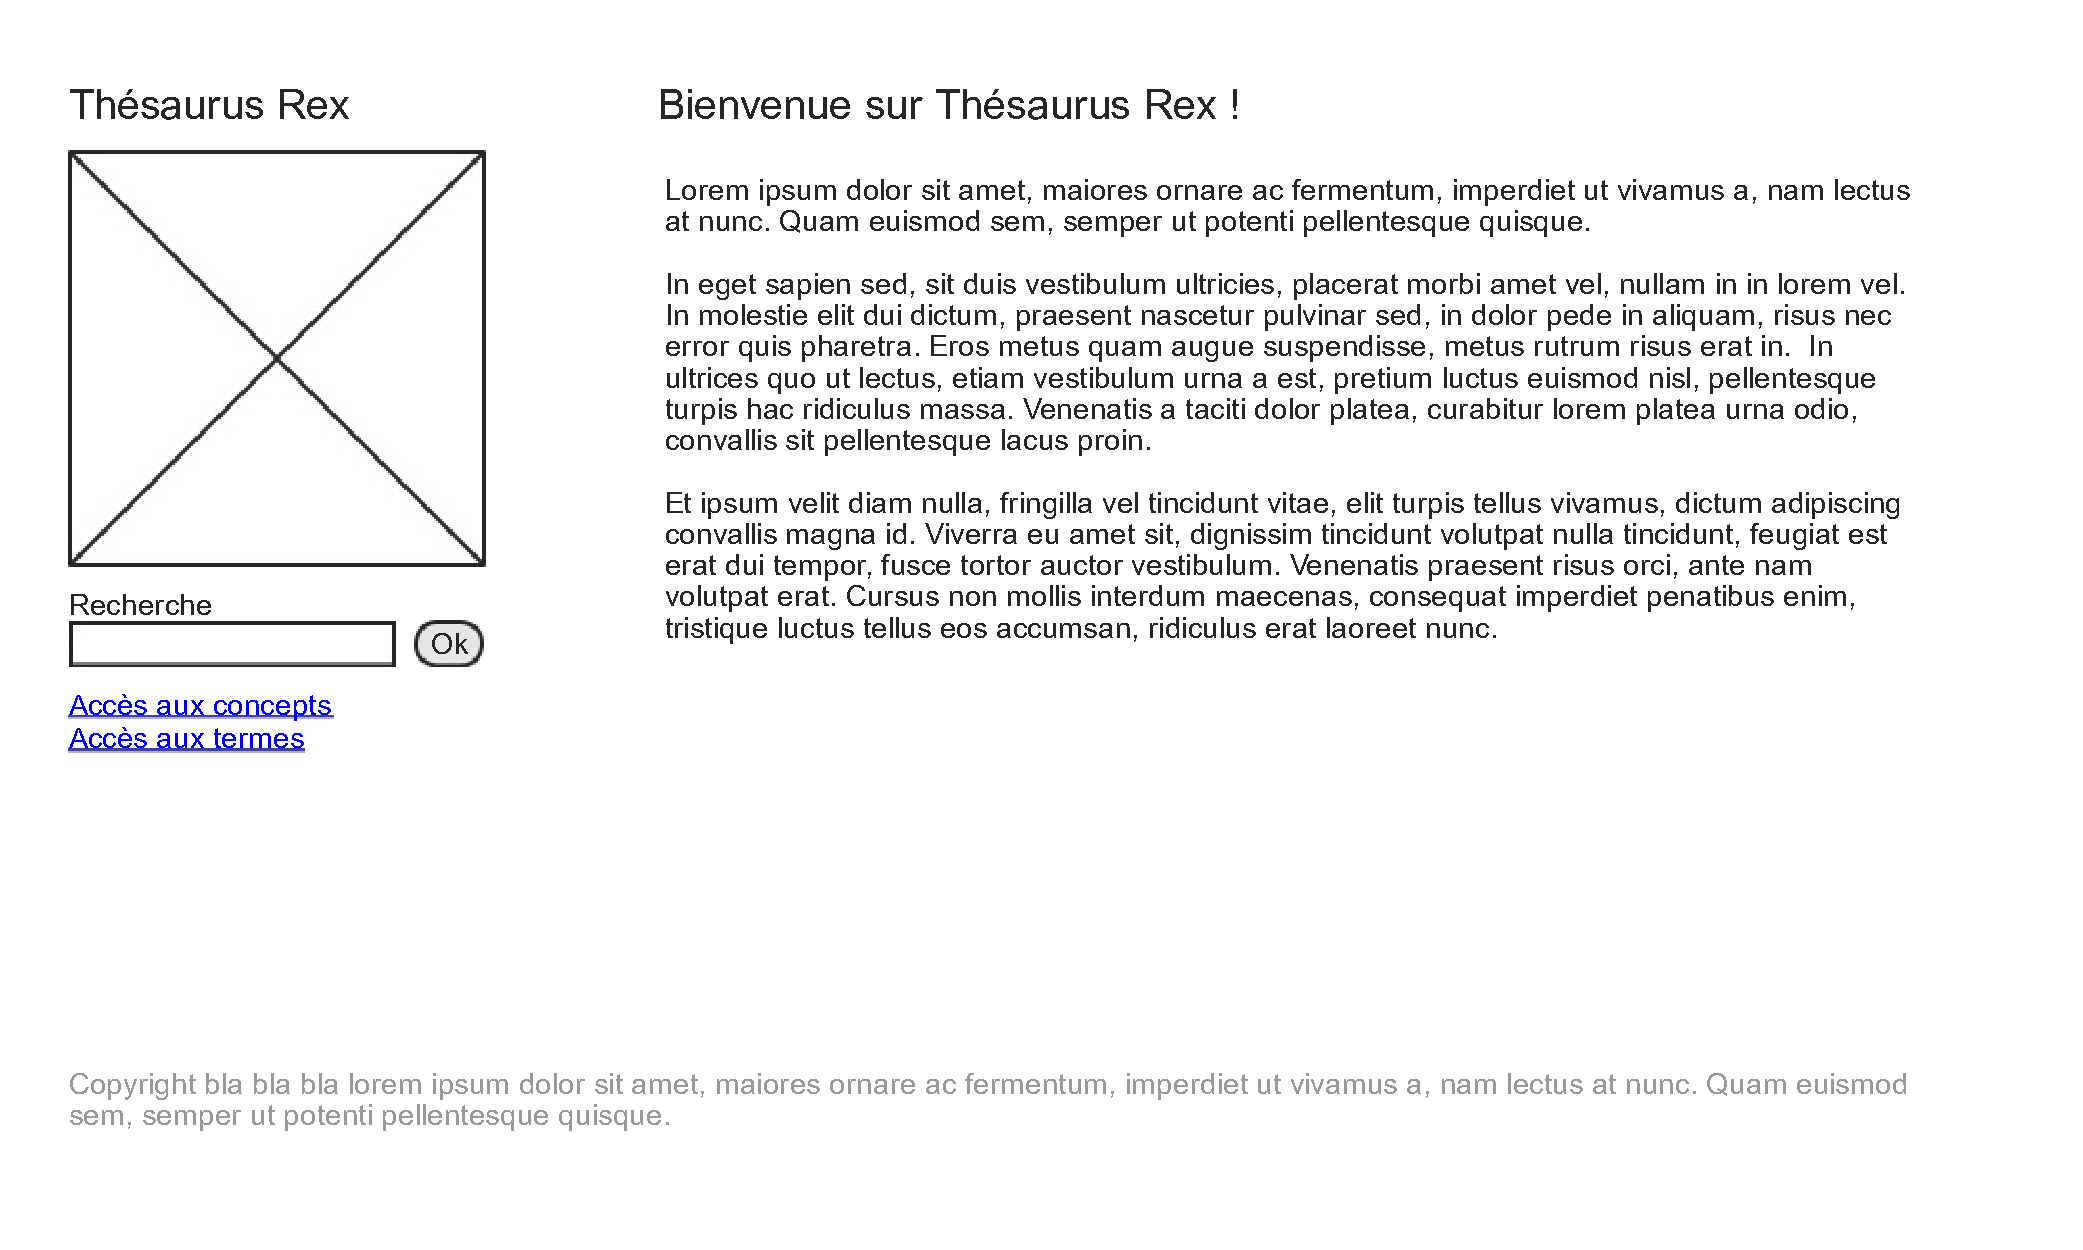
\includegraphics[width=\textwidth]{files/template_accueil}
\end{center}
\caption{Template de la page d'accueil de Thésaurus Rex.}
\end{figure}

\subsubsection{Vue hiérarchique des concepts}
\begin{figure}[H]
\begin{center}
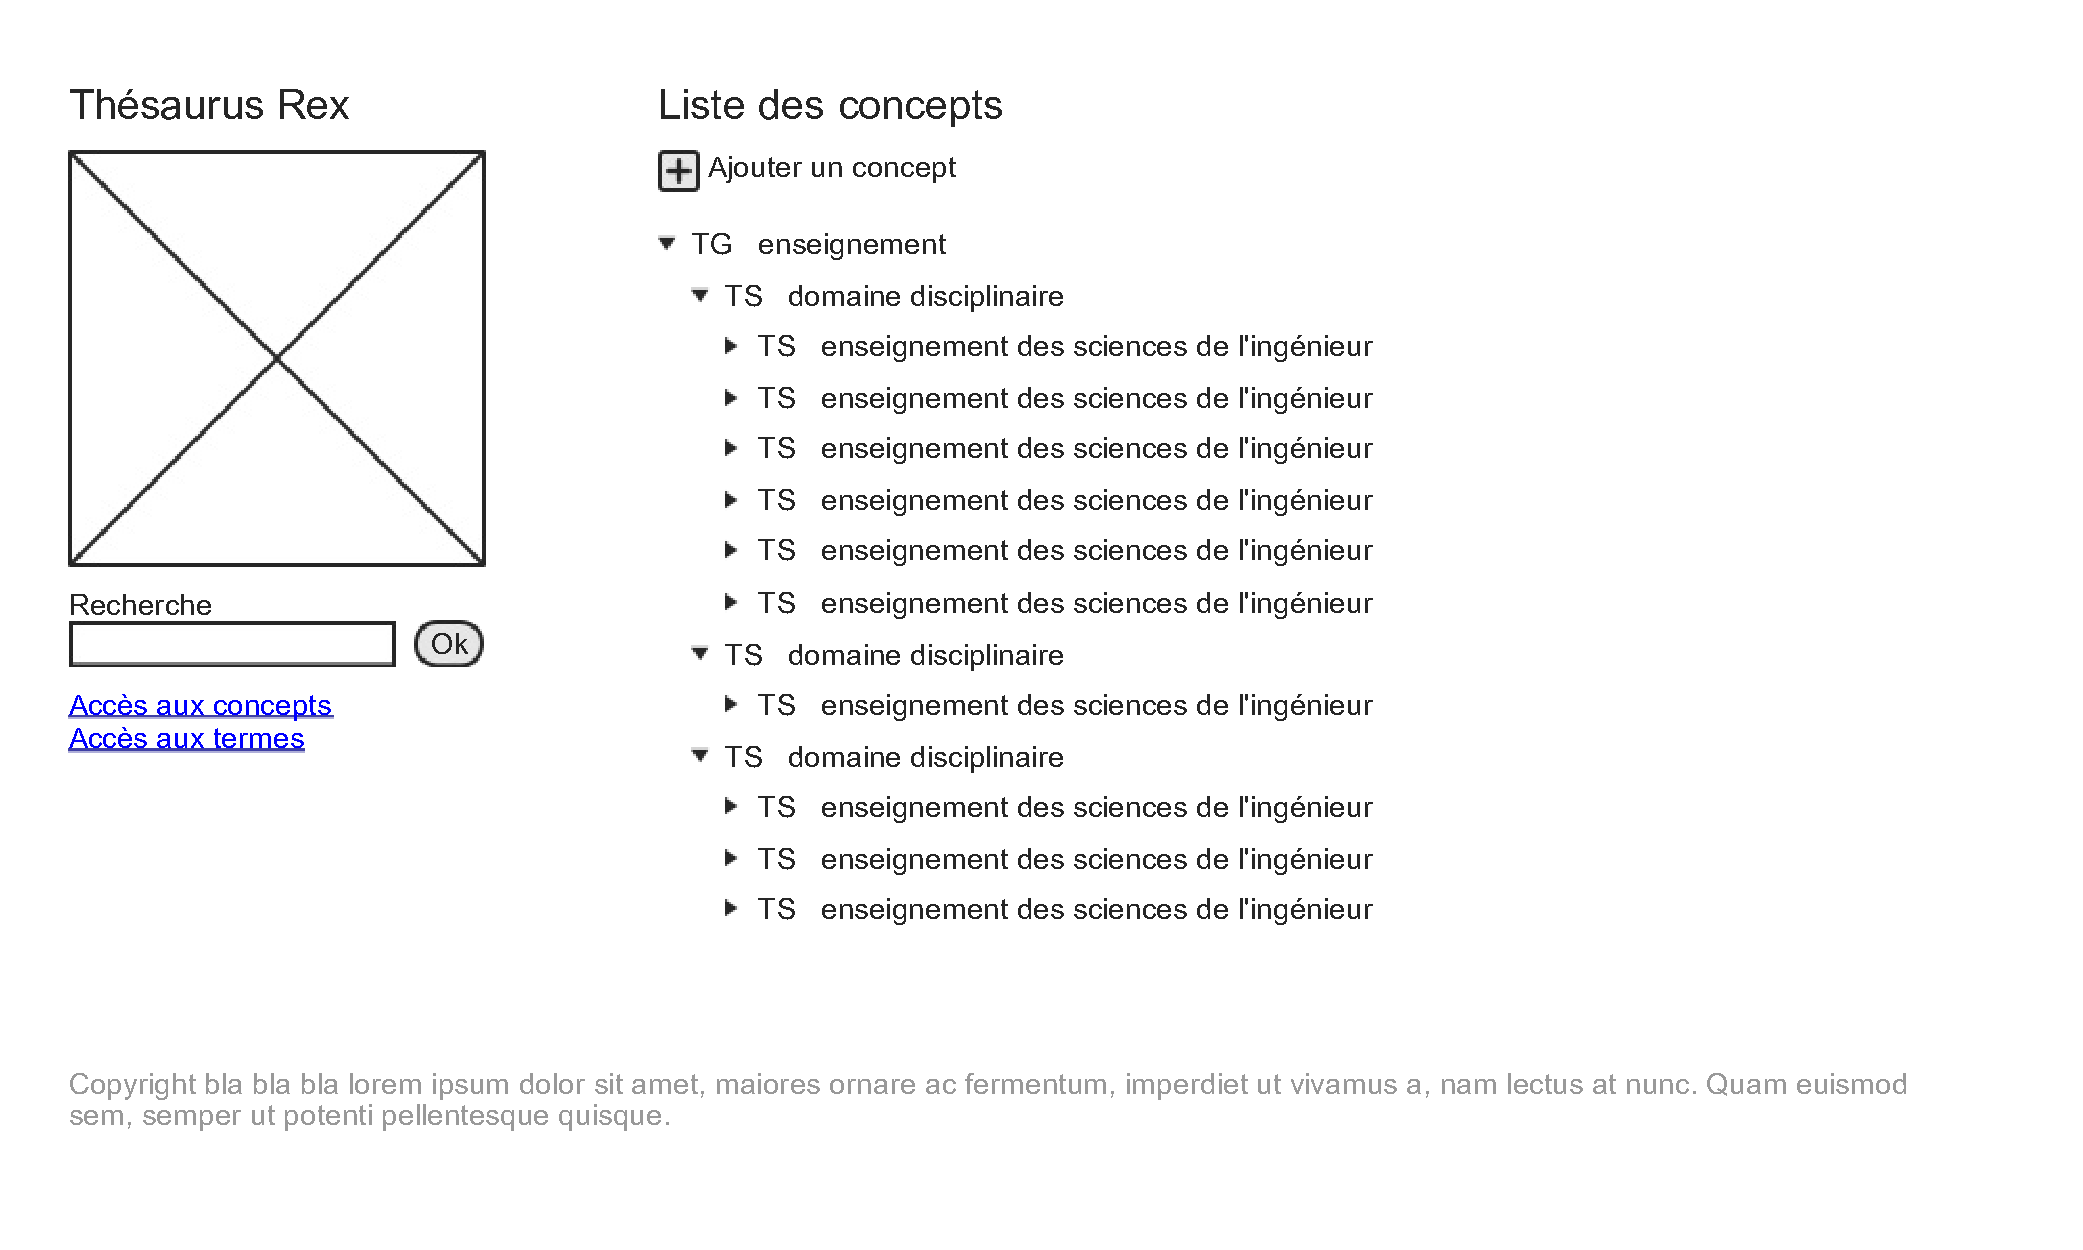
\includegraphics[width=\textwidth]{files/template_concepts}
\end{center}
\caption{Template de la vue hiérarchique des concepts.}
\end{figure}

\subsubsection{Visualisation d'un concept}
\begin{figure}[H]
\begin{center}
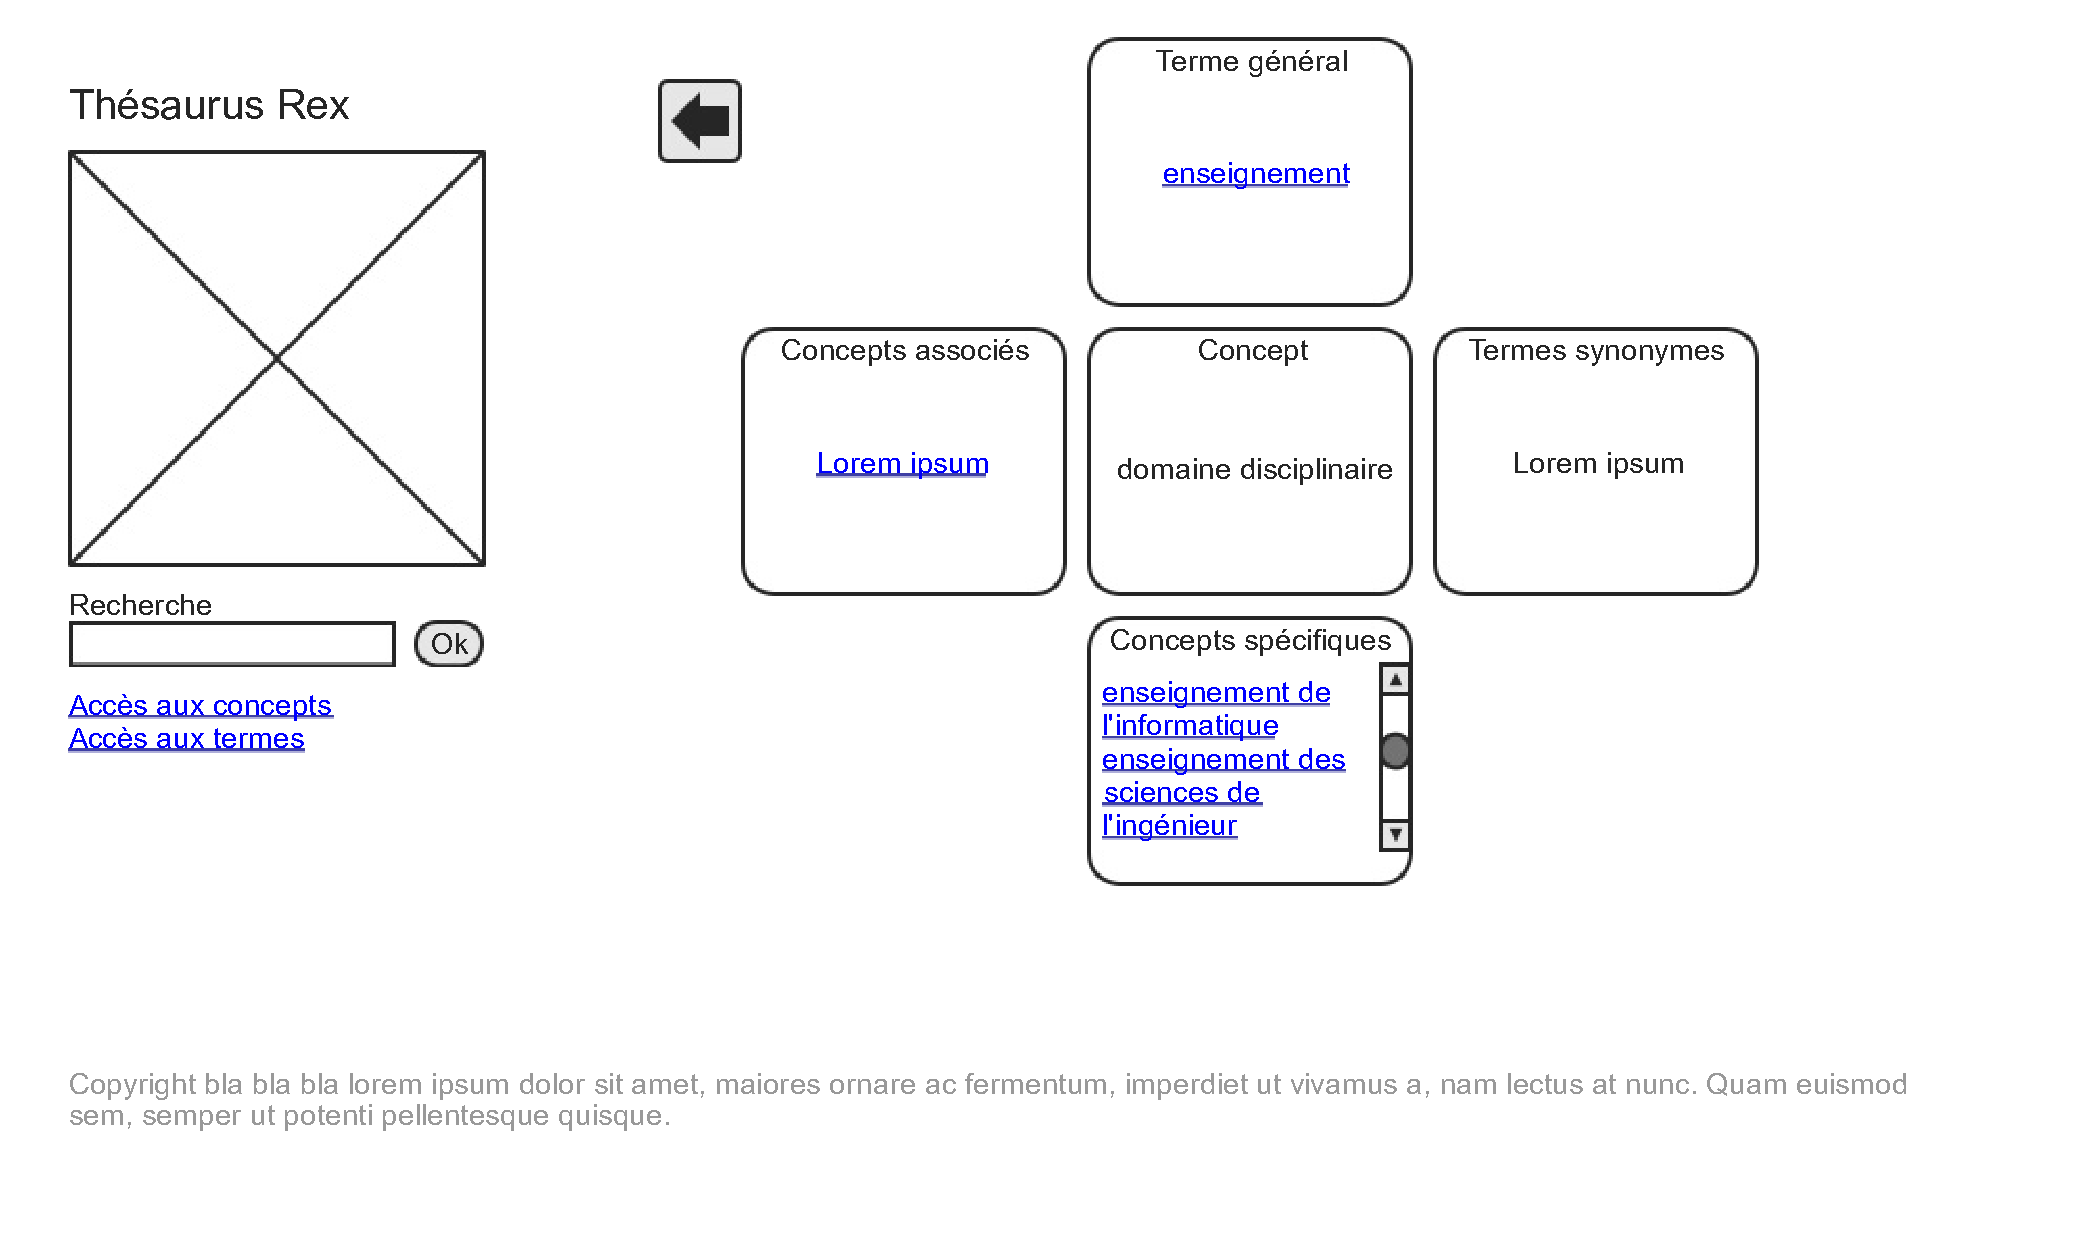
\includegraphics[width=\textwidth]{files/template_concept}
\end{center}
\caption{Template d'affichage d'un concept.}
\end{figure}

\subsubsection{Ajout / Édition d'un concept}
\begin{figure}[H]
\begin{center}
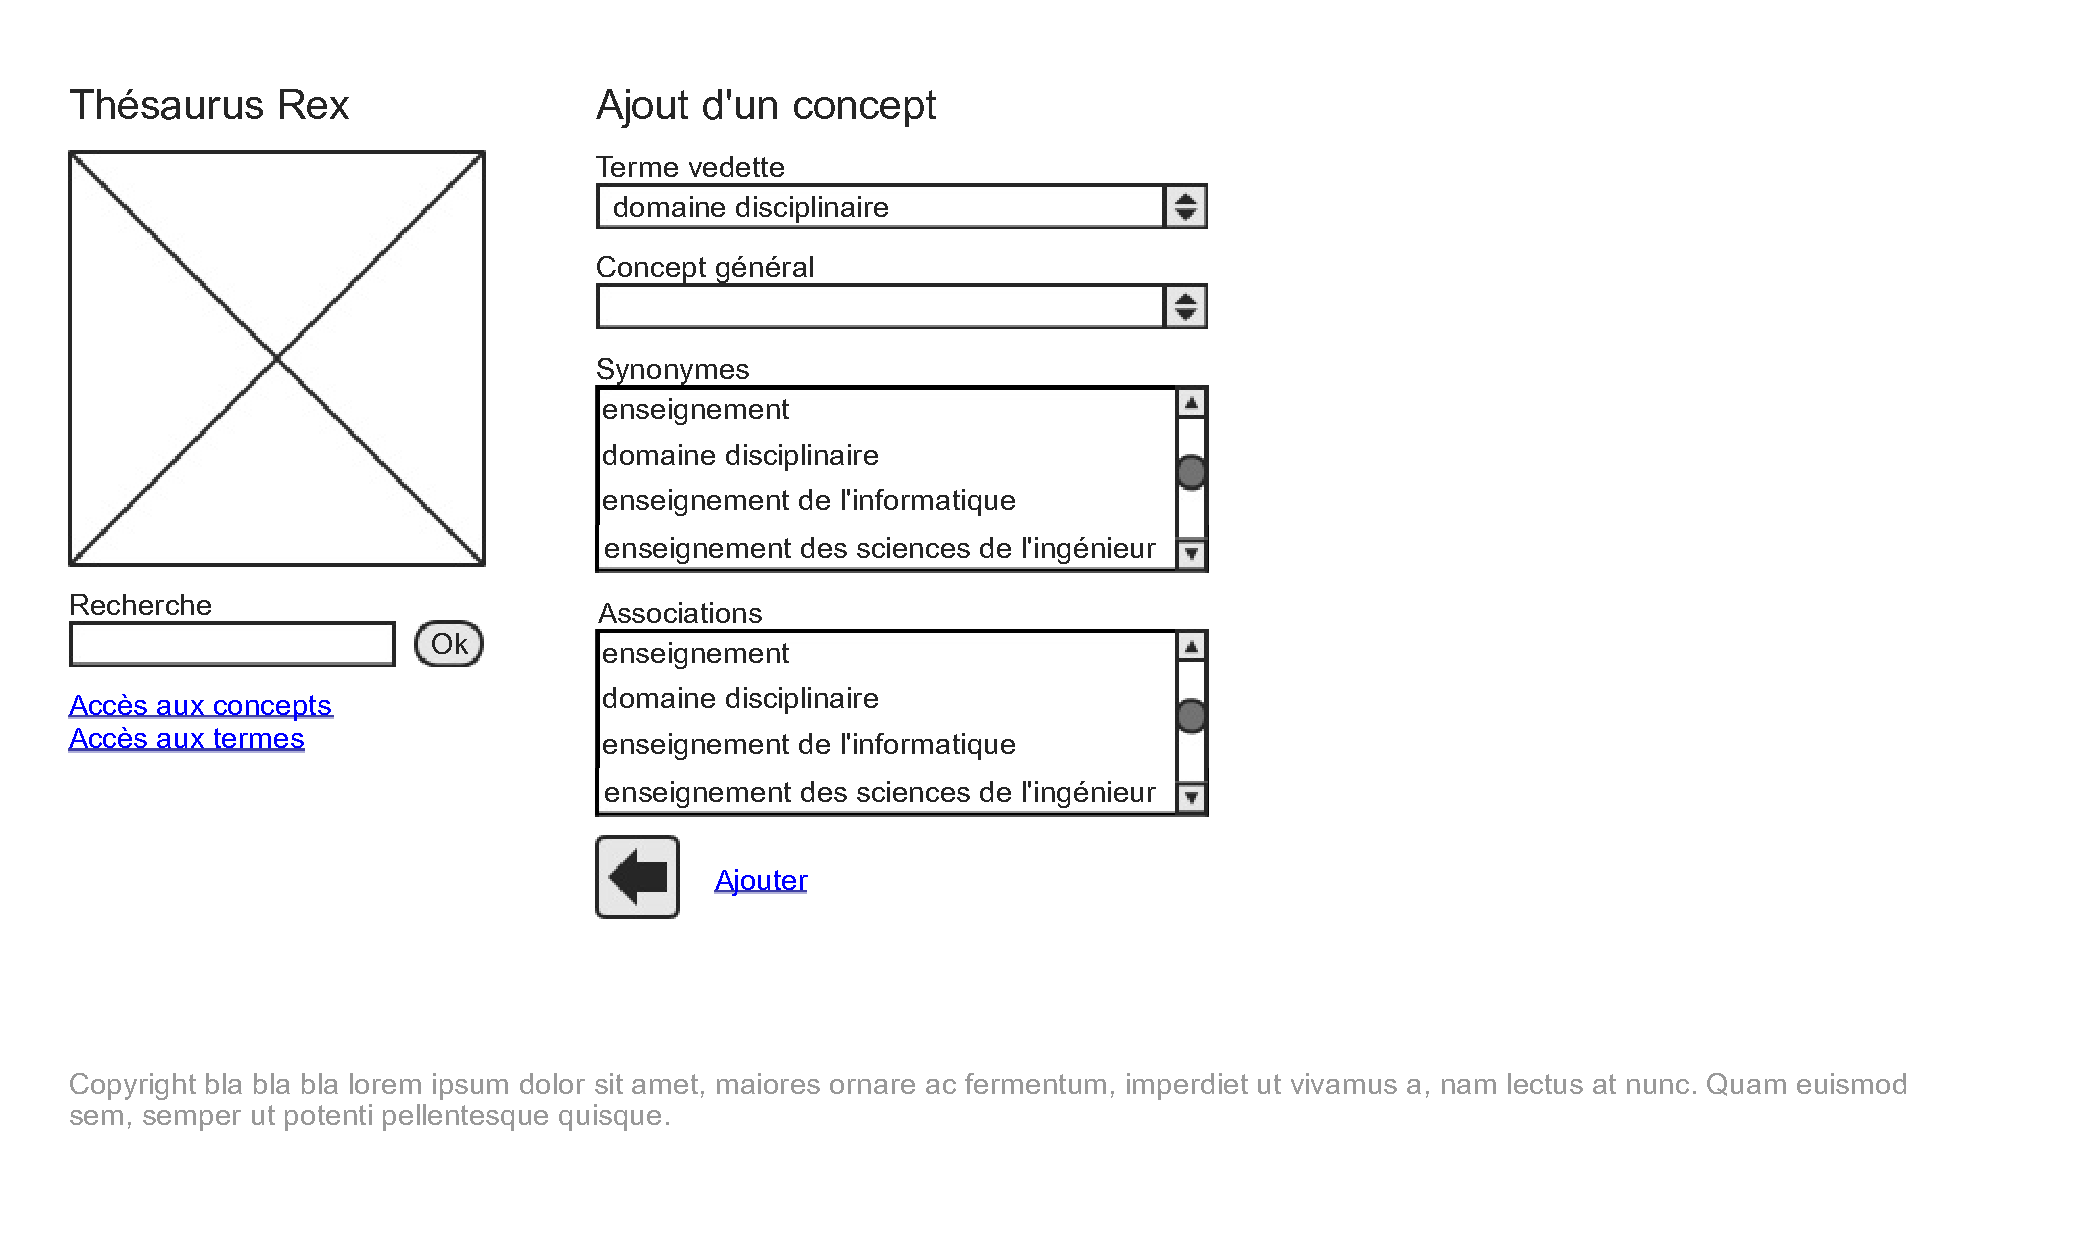
\includegraphics[width=\textwidth]{files/template_concept_add}
\end{center}
\caption{Template du formulaire d'ajout d'un concept.}
\end{figure}
\begin{figure}[H]
\begin{center}
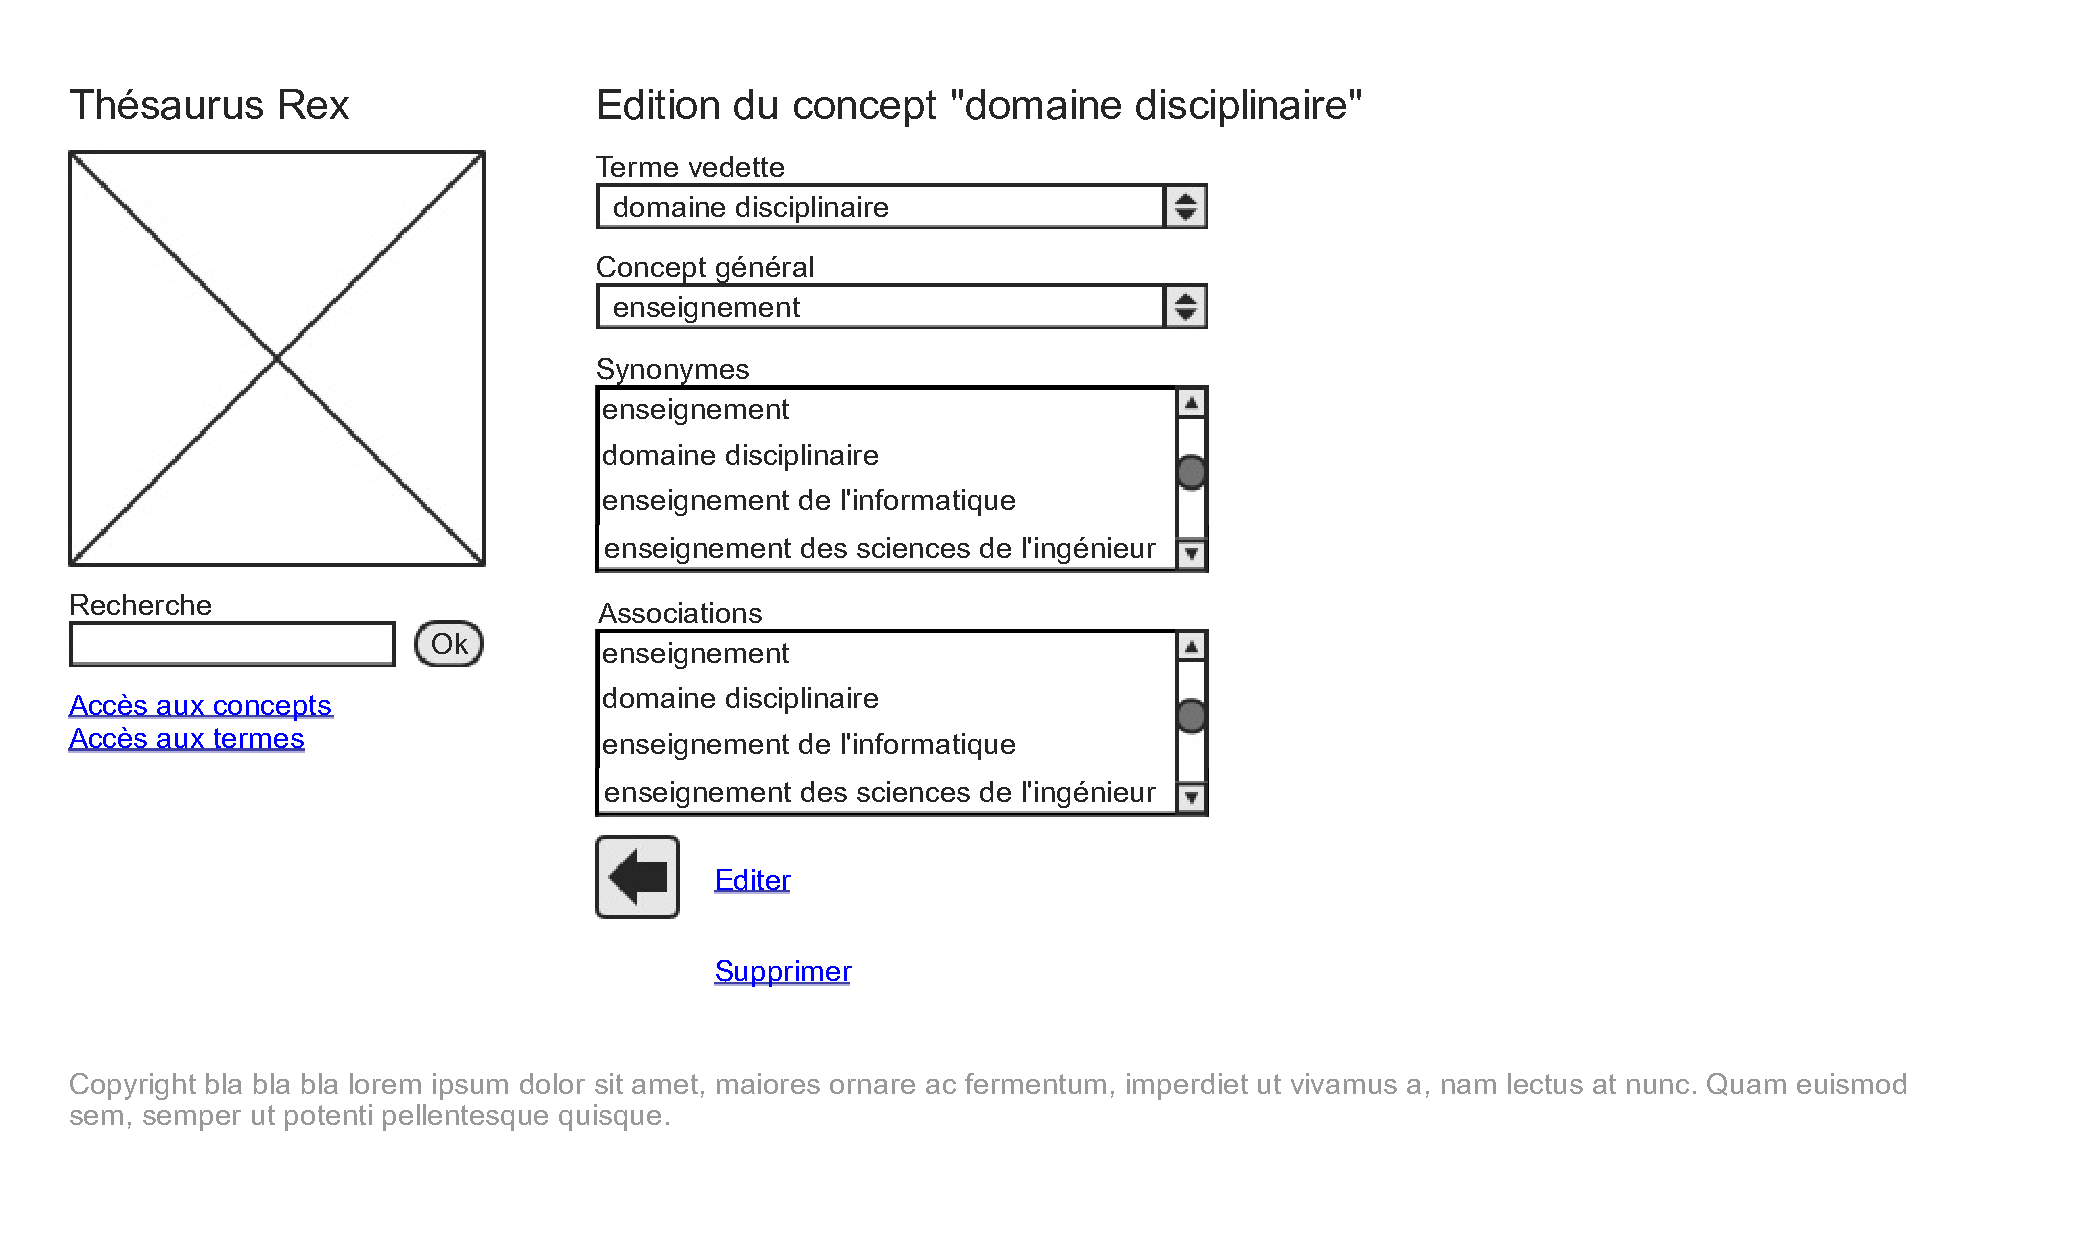
\includegraphics[width=\textwidth]{files/template_concept_edit}
\end{center}
\caption{Template du formulaire d’édition d'un concept.}
\end{figure}

\subsubsection{Liste des termes}
\begin{figure}[H]
\begin{center}
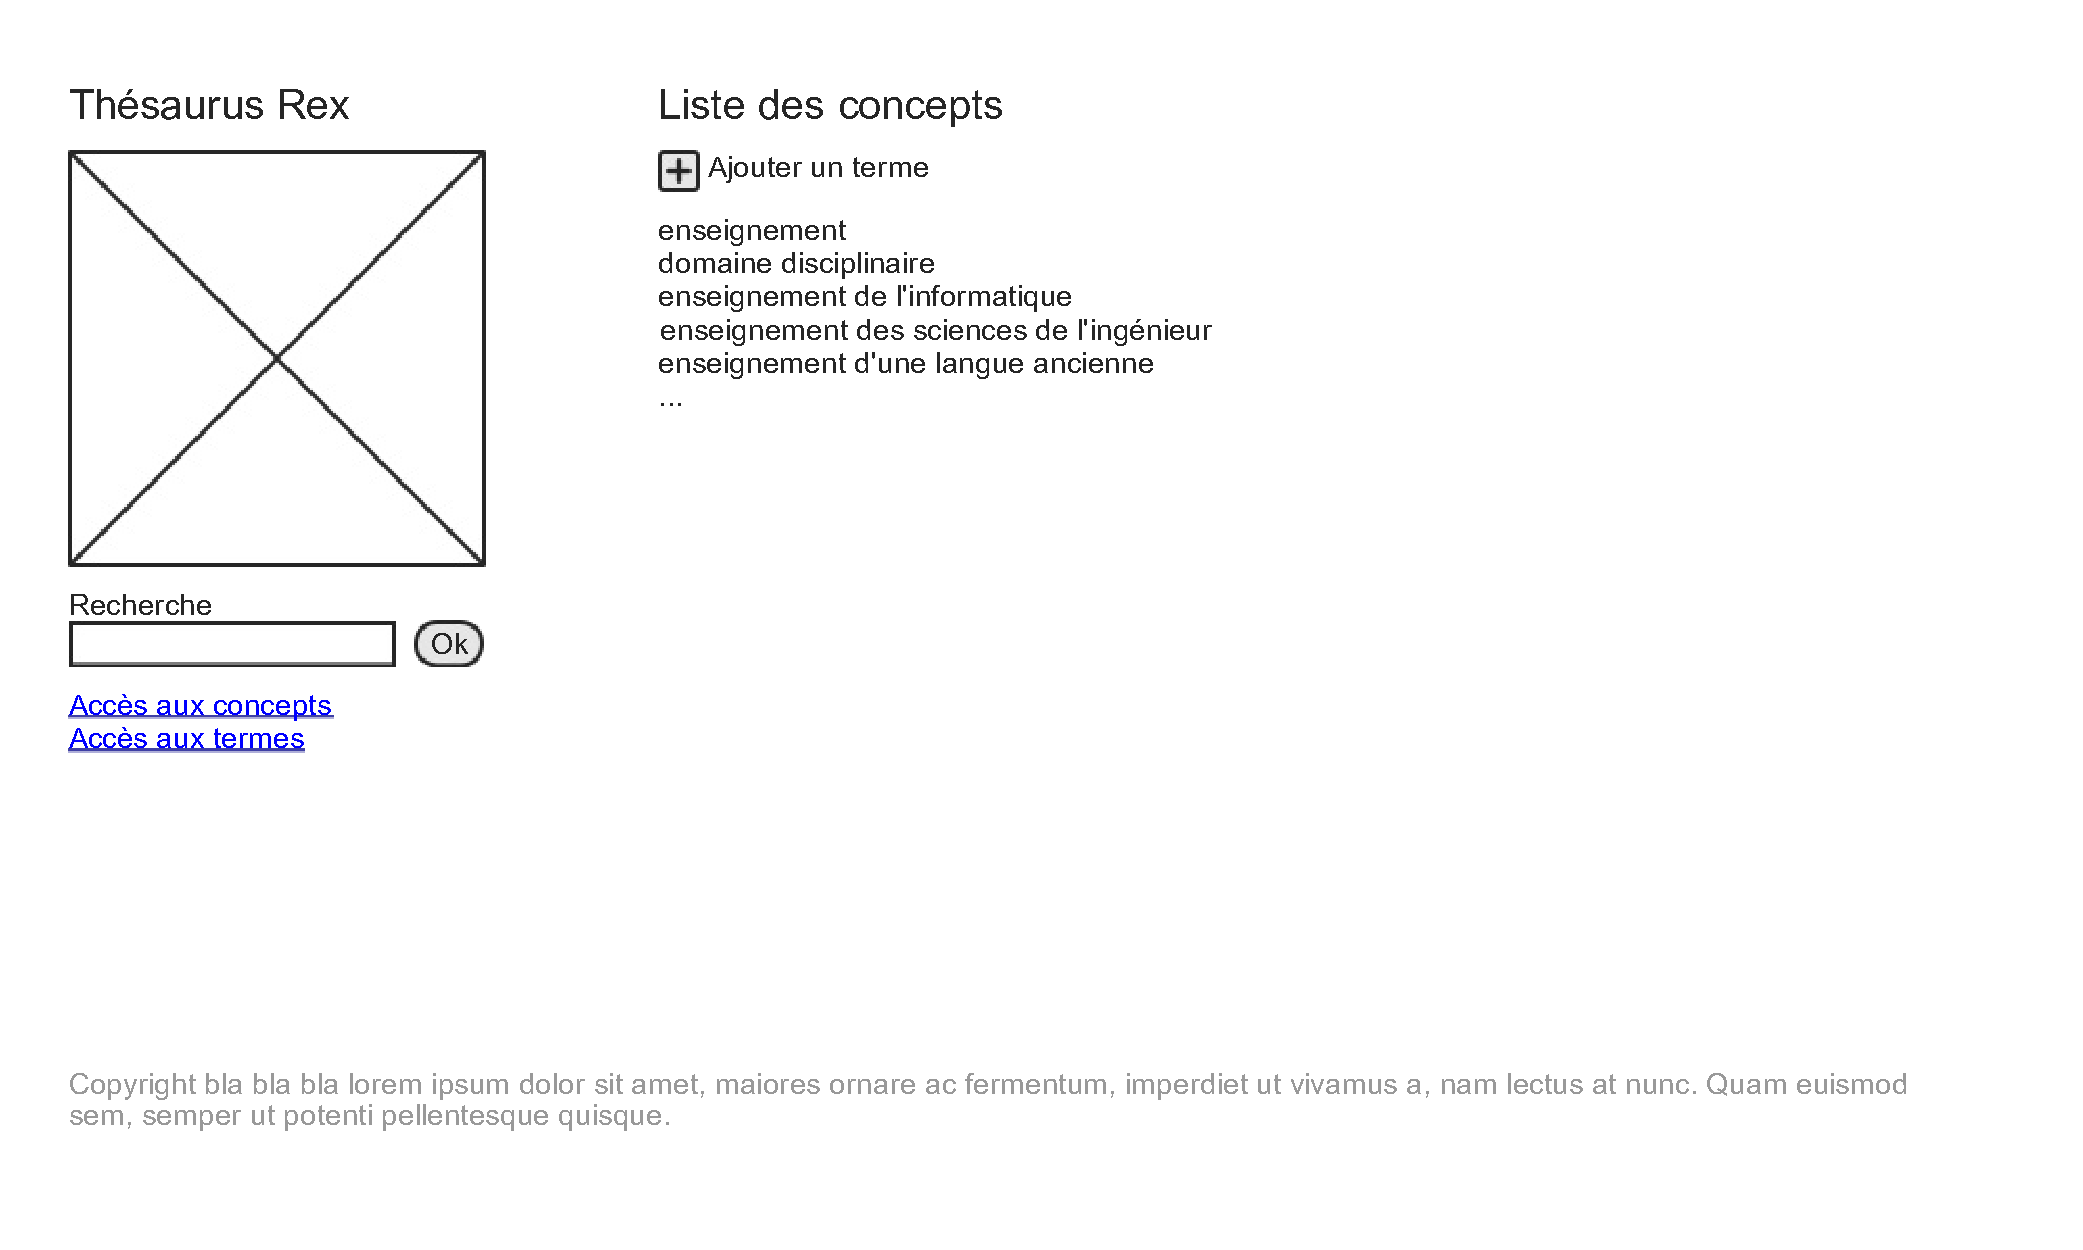
\includegraphics[width=\textwidth]{files/template_termes}
\end{center}
\caption{Template de visualisation des termes.}
\end{figure}

\subsubsection{Édition d'un terme}
\begin{figure}[H]
\begin{center}
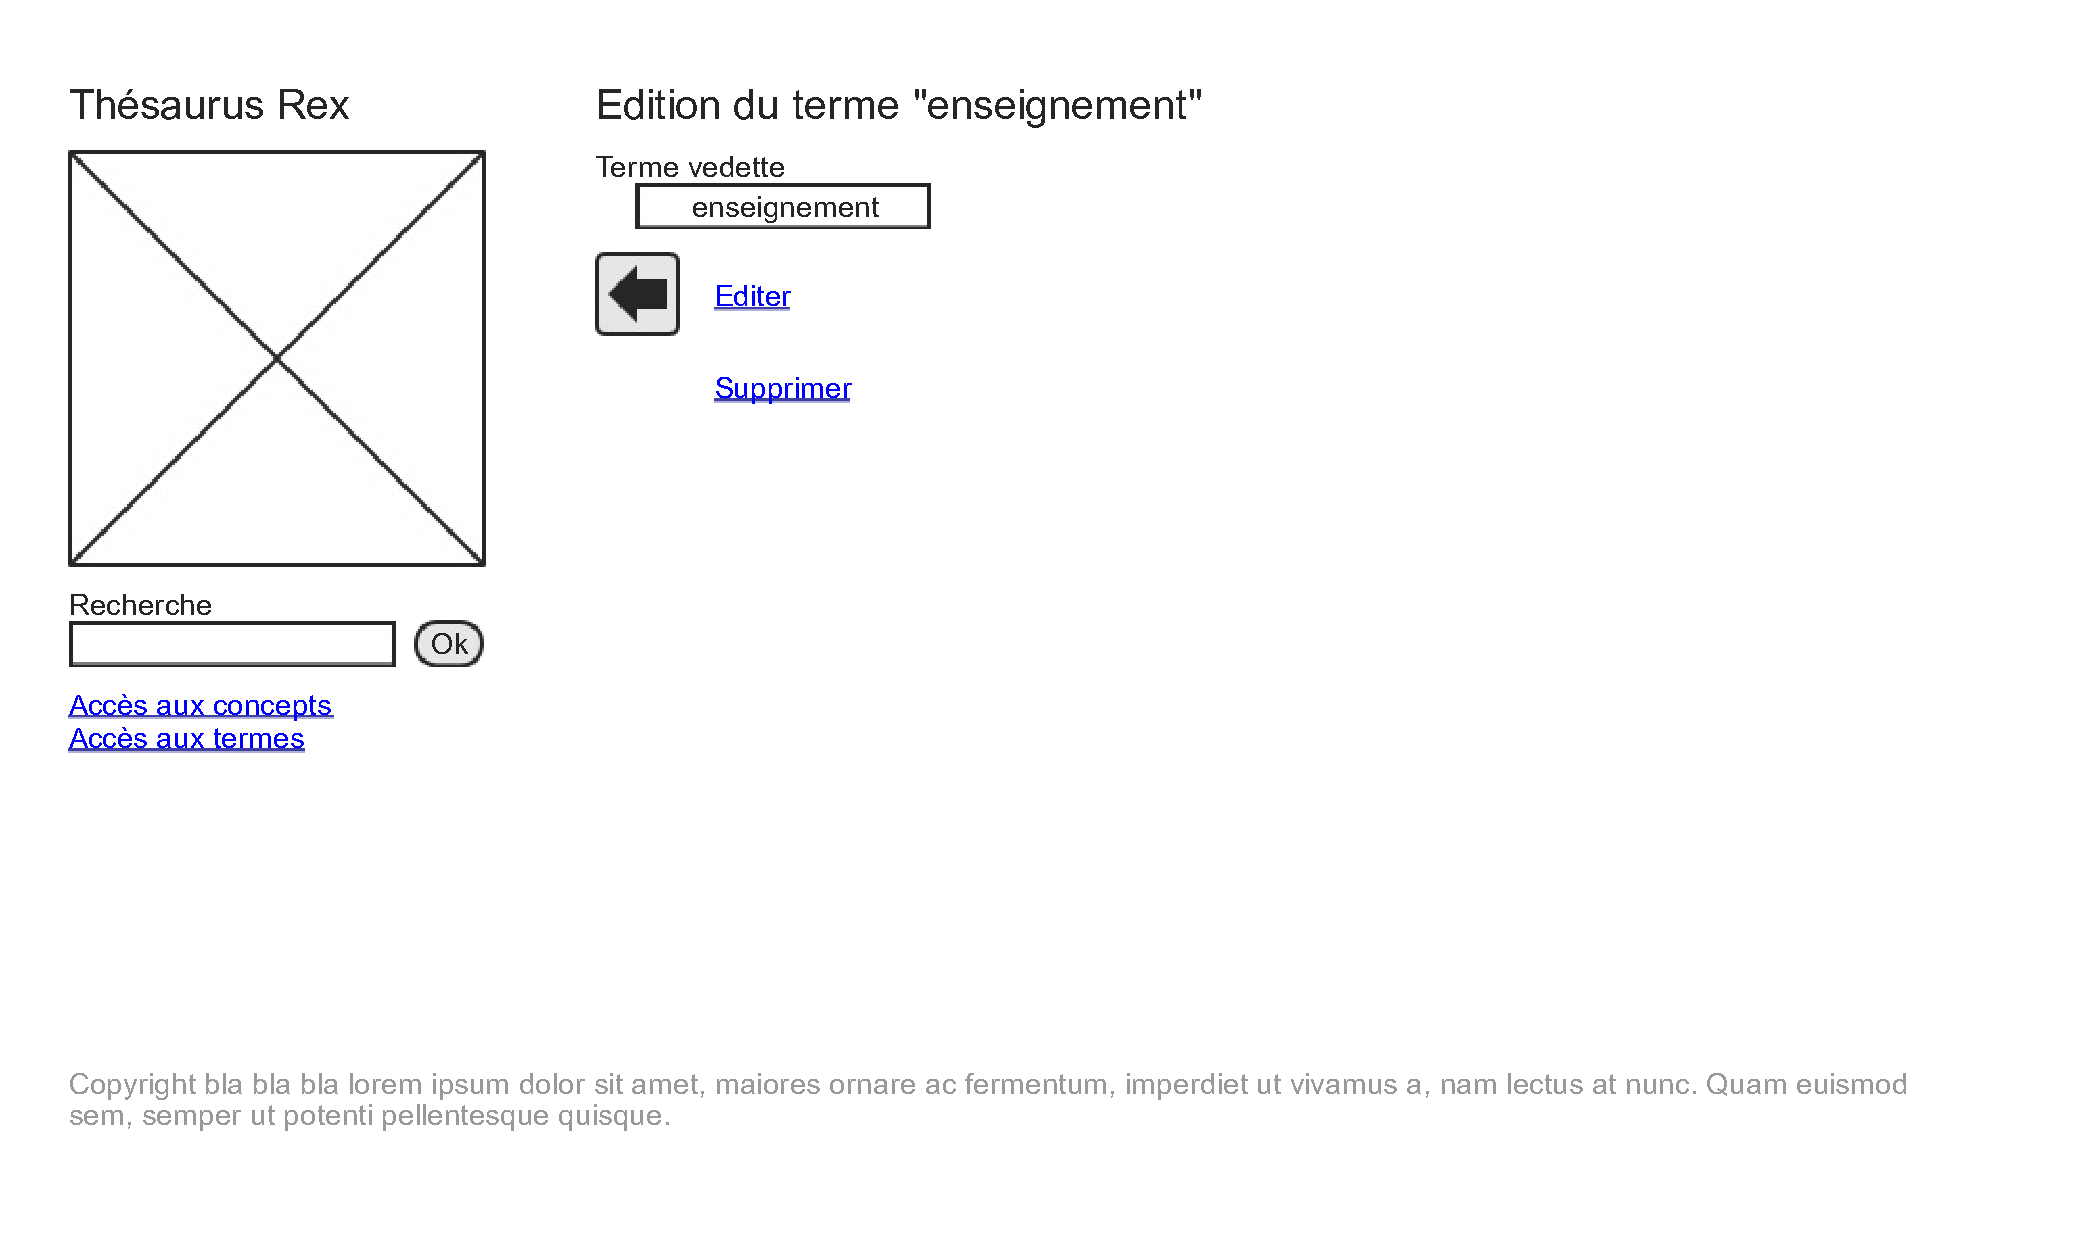
\includegraphics[width=\textwidth]{files/template_terme_edit}
\end{center}
\caption{Template du formulaire d'ajout d'un concept.}
\end{figure}


\subsection{Framework}
\chapter{Implémentation}
Classes réellement implémentées dans symfony2 + schema relationnel créé par doctrine.

Aperçus d'écran finaux

\section{Le framework Symfony2}
\subsection{Présentation du framework}
Symfony est un framework PHP développé par l'équipe française SensioLabs dirigée par Fabien Potencier. Le but d'un tel outil est d’accélérer le développement et l'accélération d'applications web en se basant sur MVC\footnote{Modèle Vue Contrôleur}, modèle classiquement utilisé dans les applications modernes.

Il s'agit d'un outil open source qui rassemble divers projets reconnus (Movaji pour le coté MVC, Doctrine pour la partie ORM, Twig pour le moteur de template).

Le projet, créé en 1998, a atteint aujourd'hui une grande maturité. Pour preuve l'utilisation de ce framework par Yahoo et Dailymotion.

Pour ce projet, nous avons utilisé la deuxième version de Symfony (Symfony2).

\subsection{Structure des applications}

\subsubsection{Bundle}
Il s'agit d'un module ou d'un plugin :
\begin{itemize}
\item portable,
\item facilement installable dans un projet Symfony2,
\item qui possède une architecture MVC.
\end{itemize}

Un bundle ne possède pas de définition exacte. Il peut être vu comme un projet à part entière, une partie d'un projet, un plugin, etc\ldots

Chaque Bundle possède des vues, des entitées, des contrôleurs, etc\ldots

\subsubsection{Entity}
Une entité (Entity) est une classe présente dans un Bundle. Elle peut être en relation avec l'ORM afin d'être persistante, posséder des formulaires, être associée à des actions ou à des vues.

\subsection{L'ORM Doctrine2}

Doctrine2 est un des ORM le plus utilisé à ce jour. Il est sous licence libre GNU LGPL. C'est l'ORM par défaut de Symfony depuis la version 1.3. Parfaitement intégré au framework, les entités créées dans les Bundles Symfony peuvent contenir des tags qui permettent de dialoguer avec Doctrine et de définir la clé primaire, les relations, les types de champs, etc\ldots

\section{Structure de l'application}

Pour le développement de cette application, nous avons créé un Bundle nommé \emph{ProjetBDDThesaurusBundle}, contenant lui même les deux entités déclarées dans notre diagramme de classe final : \emph{Terme} et \emph{Concept}.

\subsection{Entité \emph{Terme}}
\lstinputlisting[language=PHP,morekeywords={class, public, function, return, private, namespace, use}]{../../App/Symfony/src/ProjetBDD/Thesaurus/Bundle/Entity/Terme.php}

\subsection{Entité \emph{Concept}}
\lstinputlisting[language=PHP,morekeywords={class, public, function, return, private, namespace, use}]{../../App/Symfony/src/ProjetBDD/Thesaurus/Bundle/Entity/Concept.php}

\section{Schéma relationnel généré}

\subsection{Schéma simplifié}
\begin{description}
\item[terme](\underline{id})
\item[concept](\underline{id}, terme\_vedette\_id\up{\#}, concept\_general\_id\up{\#}) (Impossibilité de mettre en clé primaire une clé étrangère :s)
\item[concept\_terme](\underline{concept\_id\up{\#}, terme\_id\up{\#}})
\item[concept\_concept](\underline{concept1\_id\up{\#}, concept2\_id\up{\#}})
\end{description}

\subsection{Schéma complet}
\begin{verbatim}
thibaut=> \d+ terme
                          Table « public.terme »
 Colonne |          Type          | Modificateurs | Stockage 
---------+------------------------+---------------+----------
 id      | character varying(255) | non NULL      | extended  
Index :
    "terme_pkey" PRIMARY KEY, btree (id)
Référencé par :
    TABLE "concept" CONSTRAINT "fk_28f759cce6a95e6d" FOREIGN KEY (t
erme_vedette_id) REFERENCES terme(id)
    TABLE "concept_terme" CONSTRAINT "fk_3bf6677a26062764" FOREIGN 
KEY (terme_id) REFERENCES terme(id) ON DELETE CASCADE
Contient des OID: non

thibaut=> \d+ concept
                                          Table « public.concept »
      Colonne       |          Type          |  Modificateurs   | Stockage  
--------------------+------------------------+------------------+----------
 id                 | integer                | non NULL         | plain    
 terme_vedette_id   | character varying(255) | Par défaut, NULL | extended
 concept_general_id | integer                |                  | plain     
Index :
    "concept_pkey" PRIMARY KEY, btree (id)
    "idx_28f759ccd859483c" btree (concept_general_id)
    "idx_28f759cce6a95e6d" btree (terme_vedette_id)
Contraintes de clés étrangères :
    "fk_28f759ccd859483c" FOREIGN KEY (concept_general_id) REFERENC
ES concept(id)
    "fk_28f759cce6a95e6d" FOREIGN KEY (terme_vedette_id) REFERENCES
 terme(id)
Référencé par :
    TABLE "concept" CONSTRAINT "fk_28f759ccd859483c" FOREIGN KEY (c
oncept_general_id) REFERENCES concept(id)
    TABLE "concept_terme" CONSTRAINT "fk_3bf6677af909284e" FOREIGN 
KEY (concept_id) REFERENCES concept(id) ON DELETE CASCADE
    TABLE "concept_concept" CONSTRAINT "fk_79a50ccb47f1482c" FOREIG
N KEY (concept1_id) REFERENCES concept(id)
    TABLE "concept_concept" CONSTRAINT "fk_79a50ccb5544e7c2" FOREIG
N KEY (concept2_id) REFERENCES concept(id)
Triggers :
    tgr_verif_root AFTER DELETE OR UPDATE ON concept FOR EACH ROW E
XECUTE PROCEDURE fc_verif_root()
Contient des OID: non

thibaut=> \d+ concept_terme
                        Table « public.concept_terme »
  Colonne   |          Type          | Modificateurs | Stockage 
------------+------------------------+---------------+----------
 concept_id | integer                | non NULL      | plain     
 terme_id   | character varying(255) | non NULL      | extended  
Index :
    "concept_terme_pkey" PRIMARY KEY, btree (concept_id, terme_id)
    "idx_3bf6677a26062764" btree (terme_id)
    "idx_3bf6677af909284e" btree (concept_id)
Contraintes de clés étrangères :
    "fk_3bf6677a26062764" FOREIGN KEY (terme_id) REFERENCES terme(i
d) ON DELETE CASCADE
    "fk_3bf6677af909284e" FOREIGN KEY (concept_id) REFERENCES conce
pt(id) ON DELETE CASCADE
Contient des OID: non

thibaut=> \d+ concept_concept
                Table « public.concept_concept »
   Colonne   |  Type   | Modificateurs | Stockage 
-------------+---------+---------------+----------
 concept1_id | integer | non NULL      | plain     
 concept2_id | integer | non NULL      | plain     
Index :
    "concept_concept_pkey" PRIMARY KEY, btree (concept1_id, concept2_id)
    "idx_79a50ccb47f1482c" btree (concept1_id)
    "idx_79a50ccb5544e7c2" btree (concept2_id)
Contraintes de clés étrangères :
    "fk_79a50ccb47f1482c" FOREIGN KEY (concept1_id) REFERENCES concept(id)
    "fk_79a50ccb5544e7c2" FOREIGN KEY (concept2_id) REFERENCES concept(id)
Triggers :
    tgr_gestion_relations AFTER INSERT OR DELETE OR UPDATE ON concept_concept FOR EACH ROW EXECUTE PROCEDURE fc_gestion_relations()
Contient des OID: non

\end{verbatim}

\subsection{Ajout d'un déclencheur}

Dans le but de gérer la symétrie des associations entre concepts (table \texttt{concept\_concept}), nous avons développé un déclencheur qui :
\begin{itemize}
\item lors d'un \texttt{INSERT} ajoute l'association symétrique,
\item lors d'un \texttt{UPDATE} modifie l'association symétrique correspondante,
\item lors d'un \texttt{DELETE} supprime l'association symétrique correspondante.
\end{itemize}

Ce déclencheur assure l'intégrité des relations à tout moment.

\subsubsection{Script de mise en place du déclencheur}
\lstinputlisting[language=sql,morekeywords={REPLACE,FUNCTION,RETURNS,IF,ELSEIF,RETURN,LANGUAGE,DECLARE,BEGIN,FOR,EACH,ROW,PROCEDURE}]{./sources/trigger.sql}

\section{Templates finaux}

\subsubsection{Accueil}
\begin{figure}[H]
\begin{center}
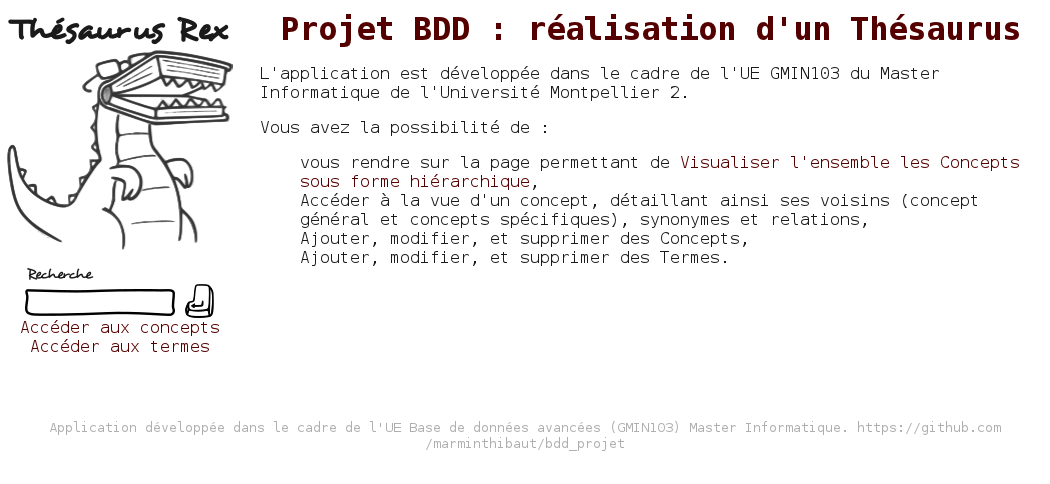
\includegraphics[width=\textwidth]{files/screen_accueil}
\end{center}
\caption{Aperçu de la page d'accueil.}
\end{figure}

\subsubsection{Liste des concepts}
\begin{figure}[H]
\begin{center}
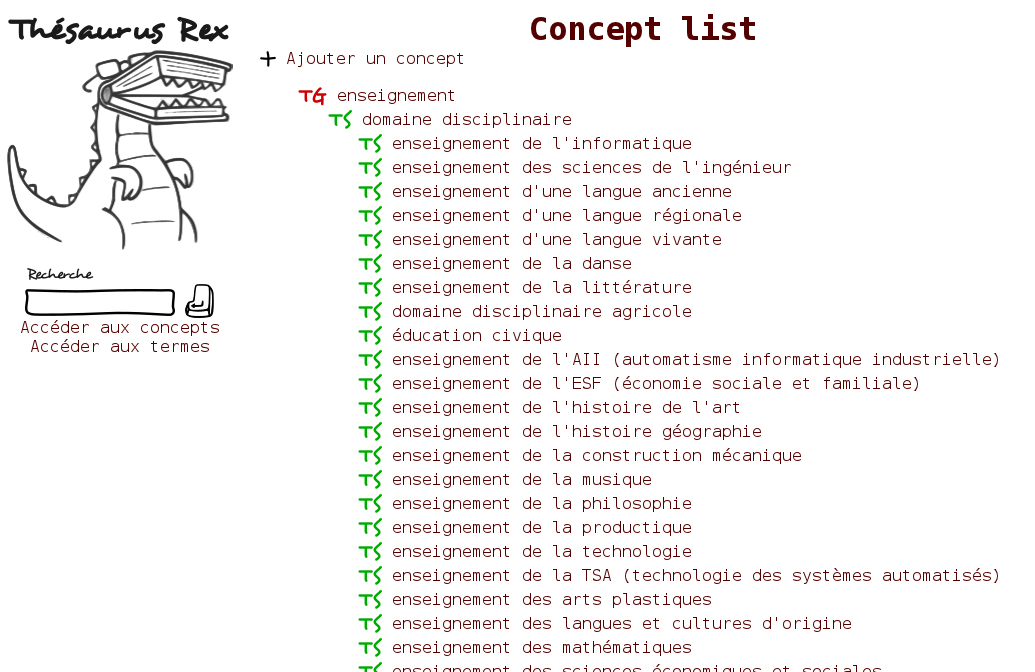
\includegraphics[width=\textwidth]{files/screen_concepts}
\end{center}
\caption{Hiérarchie des concepts.}
\end{figure}

\subsubsection{Affichage d'un concept}
\begin{figure}[H]
\begin{center}
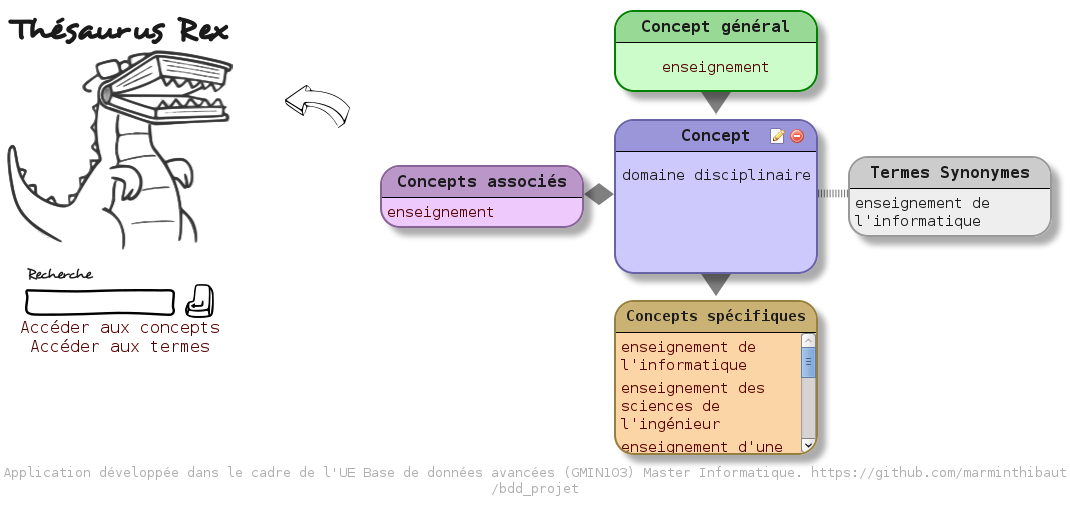
\includegraphics[width=\textwidth]{files/screen_concept}
\end{center}
\caption{Aperçu de la page d'un concept.}
\end{figure}

\subsubsection{Modification d'un concept}
\begin{figure}[H]
\begin{center}
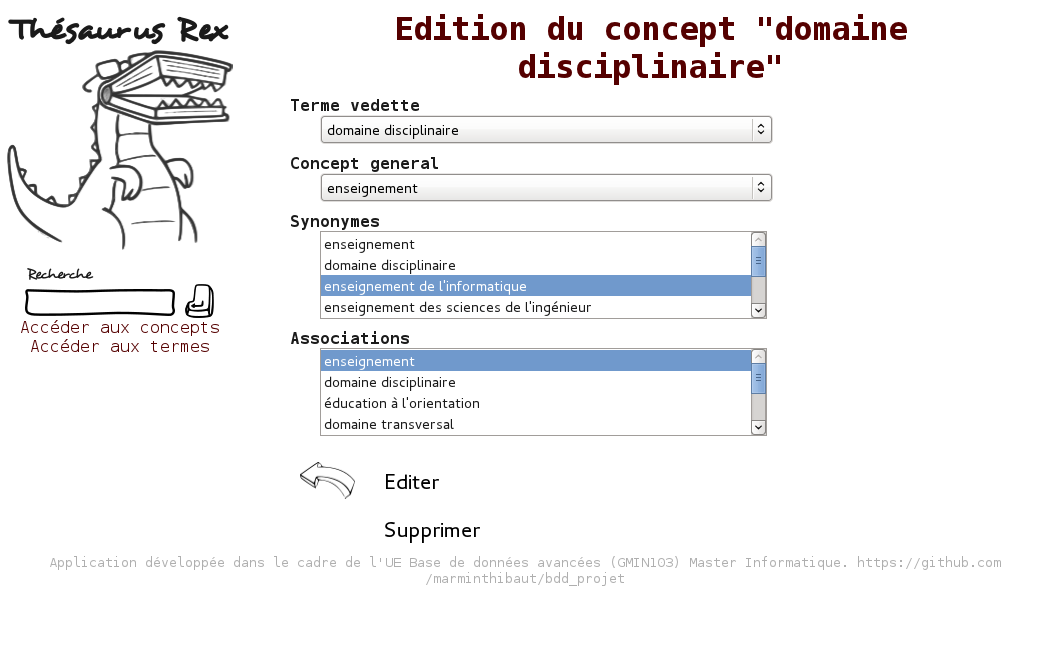
\includegraphics[width=\textwidth]{files/screen_concept_edit}
\end{center}
\caption{Formulaire de modification d'un concept.}
\end{figure}

\subsubsection{Liste des termes}
\begin{figure}[H]
\begin{center}
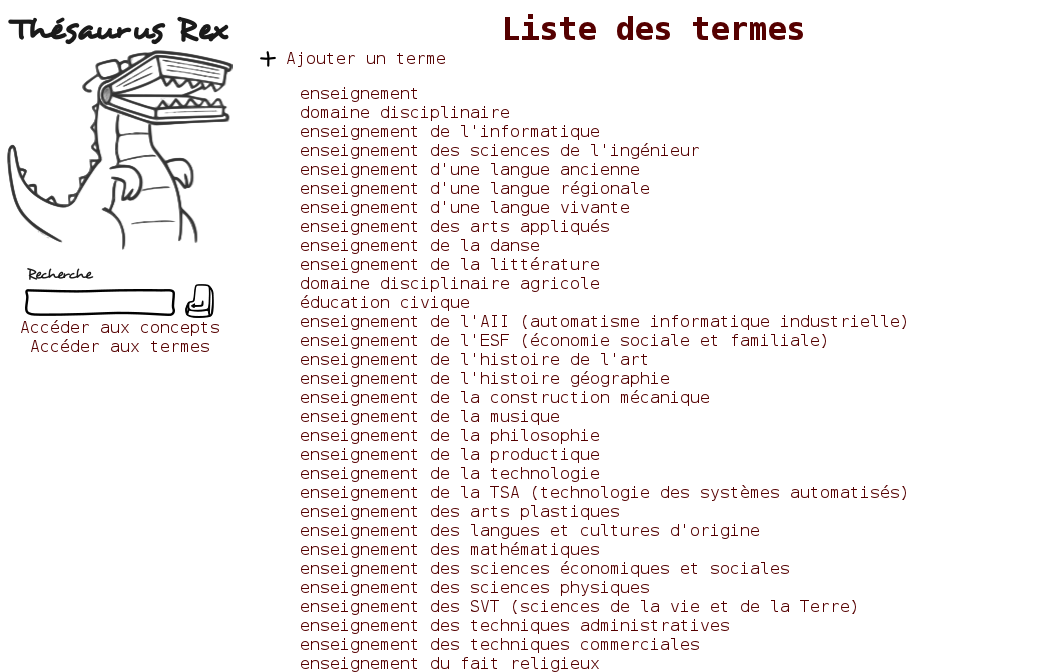
\includegraphics[width=\textwidth]{files/screen_termes}
\end{center}
\caption{Aperçu de la page de liste des termes.}
\end{figure}

\subsubsection{Modification d'un terme}
\begin{figure}[H]
\begin{center}
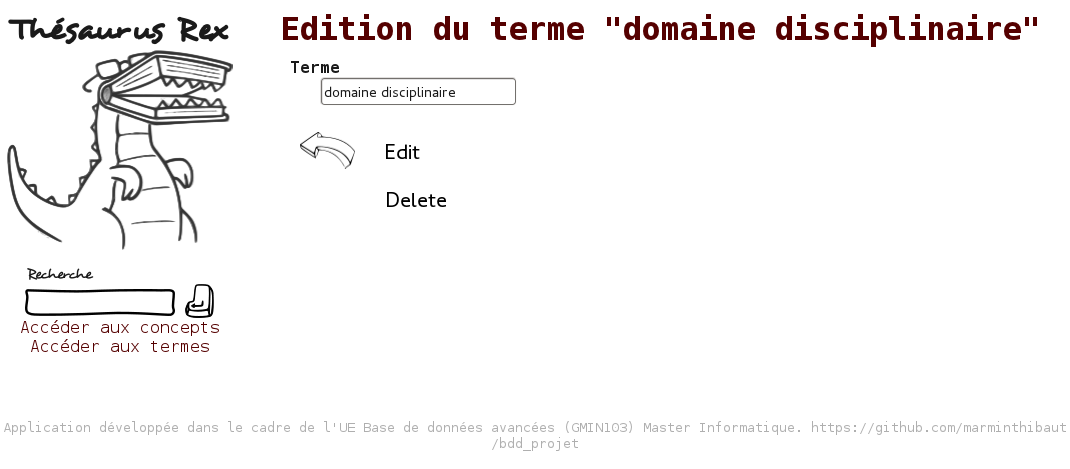
\includegraphics[width=\textwidth]{files/screen_terme_edit}
\end{center}
\caption{Formulaire d'édition d'un terme.}
\end{figure}
\end{document}
